\documentclass{article}[a4paper]
\usepackage[a4paper, total={6in, 9.5in}]{geometry}
\usepackage{charter}
\usepackage{xcolor}
\usepackage{graphicx}
\usepackage{float}
\usepackage{listings}
\usepackage{tabularray}
\usepackage{amsmath}
\usepackage{amssymb}
\usepackage{enumitem}
\usepackage{tikz}
\usepackage[hidelinks]{hyperref}

\newcommand{\extlink}{
	
\begin{tikzpicture}[scale=0.1]
		\draw[rounded corners=0.5mm, line width=0.9pt] (-1, -1) rectangle (1, 1);
		\fill[white] (0, 0) rectangle (1.3, 1.3);
		\draw[line width=0.9pt, line cap=round] (0.15, 0.15) -- (1.3, 1.3);
		\draw[line width=0.9pt, line cap=round] (0.5, 1.3) -- (1.3, 1.3) -- (1.3, 0.5);
	\end{tikzpicture}
}

\lstset{
  language=Python,
  basicstyle=\ttfamily,
  keywordstyle=\color{blue},
  commentstyle=\color{gray},
  stringstyle=\color{red},
  showstringspaces=false,
  columns=fullflexible,
  breaklines=true,
  captionpos=b,
  backgroundcolor=\color[rgb]{0.96,0.96,0.96},
  xleftmargin=6pt,
  frame=tlbr,
  framesep=6pt,
  framerule=0pt,
  aboveskip=4pt
}

\title{
	\huge{\textbf{
		Assignment 01
	}}\\
	\Large{
		Learning from Data, Related Challenges, Linear Models for Regression
	}\\
	\large{\phantom{}}\\
	\large{
		submitted for
	}\\
	\LARGE{
		\textbf{EN3150 - Pattern Recognition}
	}\\
	\large{
		Department of Electronic and Telecommunication Engineering
	}
	\\
	\large{University of Moratuwa}
}

\author{
	\textbf{Udugamasooriya P. H. J.}\\
	220658U\\
	\small{Progress on \href{https://github.com/pulasthi-u/en3150-assignment01}{GitHub \extlink}}
}

\date{20 August 2025}

\allowdisplaybreaks
\setlength{\parindent}{0pt}

\begin{document}

	\maketitle

	\section{Impact of Outliers on Linear Regression}

	\textbf{Question 02}
	We represent the independent variables in a matrix \[
		\mathbf{X} = \begin{pmatrix}
			1		& x_1		\\
			\vdots	& \vdots	\\
			1		& x_n
		\end{pmatrix},
	\] the dependent variables in a vector \[
		\mathbf{y} = \begin{pmatrix}
			y_1 & \cdots & y_n
		\end{pmatrix} ^ \top,
	\] and directly use the result that \[
		\mathbf{w}_\text{OLS}
		= \begin{pmatrix} w_0 & w_1 \end{pmatrix} ^ \top
		= \underset{\mathbf{w}}{\arg\min} \left( \mathbf{y} - \mathbf{X} \mathbf{w} \right)^2
		= \left( \mathbf{X}^\top \mathbf{X} \right)^{-1} \mathbf{X}^\top \mathbf{y}.
	\]
	
	This is exactly what we implement in the code in Listing \ref{q1_2_code}, and the results obtained
	from it are as follows:
	\begin{verbatim}
Ordinary Least Squares Weights (w): [ 3.91672727 -3.55727273]
	\end{verbatim}

	Hence, \[
		\mathbf{w}_\text{OLS} = \begin{pmatrix} 3.91672727 \\ -3.55727273 \end{pmatrix},
	\] and the predicted linear model is \[
		y = 3.91672727 - 3.55727273 x.
	\]

	A plot of the given data points against the predicted values is shown in Figure \ref{q1_2_img}.

	\begin{figure}[H]
		\centering
		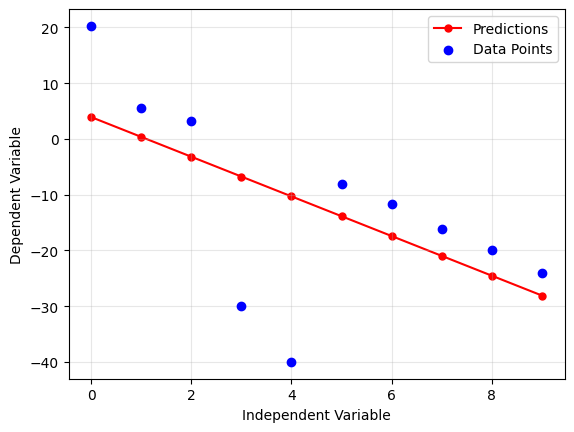
\includegraphics[width=0.9\linewidth]{images/q1_2.png}
		\caption{Given data points against predicted linear model}
		\label{q1_2_img}
	\end{figure}

	\textbf{Question 04} The code in Listing \ref{q1_4_code} was used to calculate the loss for each model for
	each given value of $\beta$. The output of the code was the following:
\begin{verbatim}
Model 1 : [12 -4]
	 Loss for beta = 1      : 0.435416262490386
	 Loss for beta = 1e-06  : 0.9999999998258207
	 Loss for beta = 1000.0 : 0.0002268287498440988
Model 2 : [ 3.91 -3.55]
	 Loss for beta = 1      : 0.9728470518681676
	 Loss for beta = 1e-06  : 0.9999999999999718
	 Loss for beta = 1000.0 : 0.00018824684654645654
\end{verbatim}

	Summarizing these results in a table, we have
	\begin{table}[H]
		\centering
		\begin{tblr}{
			colspec={X[1, c] X[1, c] X[1, c]},
			hlines, vlines,
			width=0.8\textwidth
		}
			$\beta$		& Model 1 Loss	& Model 2 Loss \\
			$1$			& $0.4354$		& $0.9728$ \\
			$10^{-6}$	& $0.9999$		& $1.0000$ \\
			$10^3$		& $0.0002$		& $0.0002$ \\
		\end{tblr}
		\caption{Losses for the two models each value of $\beta$}
	\end{table}

	\textbf{Question 05} We propose setting $\beta = 1$ to mitigate the impact of outliers. To see why, consider the following.
	\newline

	With very small values of $\beta$, the squared error term starts to dominate, and the loss becomes
	approximately equal to $1$, i.e., \[
		\dfrac{\left(y_i - \hat{y_i}\right)^2}{\left(y_i - \hat{y_i}\right)^2 + \beta^2}
		\approx
		\dfrac{\left( y_i - \hat{y_i} \right)^2}{\left( y_i - \hat{y_i} \right)^2}
		=
		1,
	\] making the result almost independent of the model used, and making it difficult to distinguish
	between several models.
	\newline
	% tend to force the squared error term to become very small. In the presence
	% of outliers, a model that closely approximates the behavior of the inliers would produce very large
	% squared errors for the outliers, dominating the loss function. If we try to force the squared errors
	% to be as small as possible then, the model would have to settle somewhere between the inliers and outliers,
	% significantly away from the true model, just so that the error to the outliers is small enough.
	
	Very large values of $\beta$ would cause the loss to be approximately proportional to the squared error and
	very close to $0$, i.e., \[
		\dfrac{\left( y_i - \hat{y_i} \right)^2}{\left( y_i - \hat{y_i} \right)^2 + \beta^2}
		\approx
		\dfrac{\left( y_i - \hat{y_i} \right)^2}{\beta^2}
		\approx
		0,
	\] again making it difficult to distinguish between models. Further, inimizing the loss in this
	case would yield approximately the same result as that of minimizing the mean squared error.
	\newline

	It can be seen from the results above that $\beta = 10^3$ is too large, as the resulting losses from both
	models are both approximately equal, and very small and close to zero, making it difficult to distinguish
	between the two models.
	\newline

	It can also be seen that $\beta = 10^{-6}$ is too small, as the resulting losses from the models are again both
	approximately equal, but this time close to $1$, leading to the same problem as above.
	\newline

	Hence, $\beta = 1$ is the best choice of the given options, as it has yielded comparable losses for both
	models.
	\newline

	\textbf{Question 06} We will fix $\beta = 1$. The loss for Model 1 then, is $0.4354$, whereas the loss
	for Model 2 is $0.9728$. Model 1 has a lower loss and is therefore the better/more suitable model.
	\newline

	Furthermore, the plots in Figure \ref{q1_4_img} show that Model 1 passes through the inliers more closely whereas Model 2 is farther away
	from the inliers (due to the influence of the outliers). This verifies that Model 1 is indeed the better model.

	\begin{figure}[H]
		\centering
		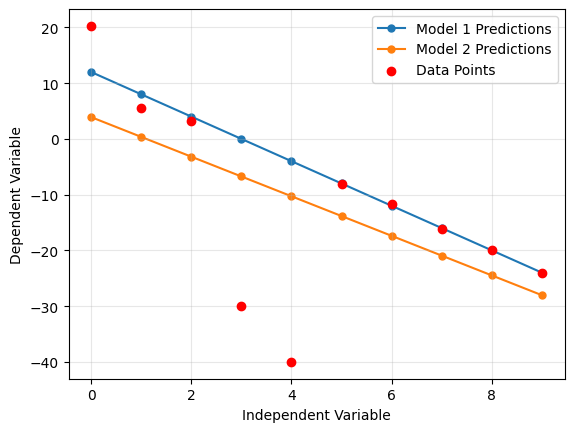
\includegraphics[width=0.9\linewidth]{images/q1_4.png}
		\caption{Comparison of Models 1 and 2}
		\label{q1_4_img}
	\end{figure}

	\textbf{Question 07} Let us start by rewriting the loss for a single data point as follows: \[
		L\left(y_i, x_i, \theta, \beta\right)
		=
		\begin{cases}
			\dfrac{1}{1 + \frac{\beta^2}{\left(y_i - \hat{y_i}\right)^2}},	& y_i \ne \hat{y_i}, \\
			0,																& \text{otherwise},
		\end{cases}
	\] where $\hat{y_i}$ is the prediction for the data point $x_i$, obtained by applying the model described by the parameters $\theta$.
	\newline
	
	Now because $\left(y_i - \hat{y_i}\right)^2 \geq 0$ for all $\hat{y_i}$, it is clear that
	$0 \leq L\left(y_i, x_i, \theta, \beta\right) < 1$ also, with small values of $\left(y_i - \hat{y_i}\right)^2$
	resulting in losses close to $0$ and large values resulting in losses close to $1$. Importantly, we observe that this property
	remains true even for outliers.
	\newline

	This has the effect of keeping the loss always restricted to a finite range, even in the presence of outliers,
	unlike with unbounded losses such as the squared error, which can grow to very large values.
	\newline
	
	Note also that because the loss due to each data point is always non-negative, the mean loss over all the data points is minimized
	when the loss from each individual data point is as small as possible.
	\newline
	
	Suppose we choose some threshold $E \in (0, 1)$ such that we would like to have \[
		\dfrac{1}{1 + \frac{\beta^2}{\left(y_i - \hat{y_i}\right)^2}} \leq E
	\] for each data point. But this is equivalent to requiring \[
		\left(y_i - \hat{y_i}\right)^2 \leq \dfrac{E}{1 - E} \cdot \beta^2,
		\quad \text{or} \quad
		\left|y_i - \hat{y_i}\right| \leq \sqrt{\dfrac{E}{1 - E}} \cdot \beta,
	\] i.e., it defines an interval of values centered around the actual value $y_i$ that the
	predicted $\hat{y_i}$ might lie within, for which the loss can still be considered ``small enough".
	\newline
	
	In this context, we can see $\beta$ acts as a hyperparameter that allows us to control how big or small the above interval is. It
	can be chosen big enough to include the distance that the outliers are away from what one might expect their true values to be.
	\newline

	Hence, with this modification in place, we prevent the outliers from introducing very large losses, and encourage
	the model to focus more on minimzing the loss due to the inliers, which significantly outnumber the outliers and thereby contribute
	more significantly to the mean loss.
	\newline

	\textbf{Question 08} Based on the nature of the outliers in the given data, we need a loss that does not completely discard them, as
	the outliers in this case still seem to follow the same general trend as the inliers and are not extremely far away from them.
	\newline
	
	Hence, a loss function that produces a significant loss for inliers, but a more slowly increasing loss for outliers is appropriate.
	\newline

	We therefore propose the Huber Loss function, defined as follows: \[
		H\left( y_i, x_i, \theta, \delta \right) = \begin{cases}
			\frac{1}{2}\left(y_i - \hat{y_i}\right)^2,										& \left|y_i - \hat{y_i}\right| \leq \delta \\
			\delta \cdot \left( \left|y_i - \hat{y_i}\right| - \frac{1}{2}\delta \right),	& \text{otherwise}.
		\end{cases}
	\] In this case, $\delta$ is a hyperparameter that determines an interval of variation for points that can be considered inliers; the Huber
	Loss is exactly the squared error for such points, but just an absolute difference for other points, i.e., outliers.

	\section{Loss Functions}

	\textbf{Question 01} We calculate the squared error \[
		\text{SE}(\hat{y_i}, y_i) = (\hat{y_i} - y_i)^2
	\] and binary cross entropy \[
		\text{BCE}(\hat{y_i}, y_i) = -y_i \log(\hat{y_i}) - (1 - y_i) \log(1 - \hat{y_i})
	\] of each predicted value $\hat{y_i}$ against the given corresponding target value $y_i$.
	\begin{table}[H]
		\centering	
		\begin{tblr}{
			colspec={X[1, c, m] X[1, c, m] X[1, c, m] X[1, c, m]},
			hlines, vlines,
			hline{Z}={1}{white},
			vline{1}={Z}{white},
			width=0.8\textwidth
		}
			True Value ($y_i$)	& Predicted Value ($\hat{y_i}$)	& $\text{SE}(\hat{y}_i, y_i)$	& $\text{BCE}(\hat{y}_i, y_i)$ \\
			$1$ 					& $0.005$ 						& $0.9900$ 						& $5.2983$ \\
			$1$ 					& $0.01$ 						& $0.9801$ 						& $4.6052$ \\
			$1$ 					& $0.05$ 						& $0.9025$ 						& $2.9957$ \\
			$1$ 					& $0.1$ 						& $0.8100$ 						& $2.3026$ \\
			$1$ 					& $0.2$ 						& $0.6400$ 						& $1.6094$ \\
			$1$ 					& $0.3$ 						& $0.4900$ 						& $1.2040$ \\
			$1$ 					& $0.4$ 						& $0.3600$ 						& $0.9163$ \\
			$1$ 					& $0.5$ 						& $0.2500$ 						& $0.6931$ \\
			$1$ 					& $0.6$ 						& $0.1600$ 						& $0.5108$ \\
			$1$ 					& $0.7$ 						& $0.0900$ 						& $0.3567$ \\
			$1$ 					& $0.8$ 						& $0.0400$ 						& $0.2231$ \\
			$1$ 					& $0.9$ 						& $0.0100$ 						& $0.1054$ \\
			$1$ 					& $1.0$ 						& $0.0000$ 						& $0.0000$ \\
									& Mean							& $0.4402$		 				& $1.4407$
		\end{tblr}
		\caption{Loss for each predicted value from both choices for the loss function}
	\end{table}
	
	A plot of the different losses against the predicted values is shown in Figure \ref{q2_1_img}.

	\begin{figure}[H]
		\centering
		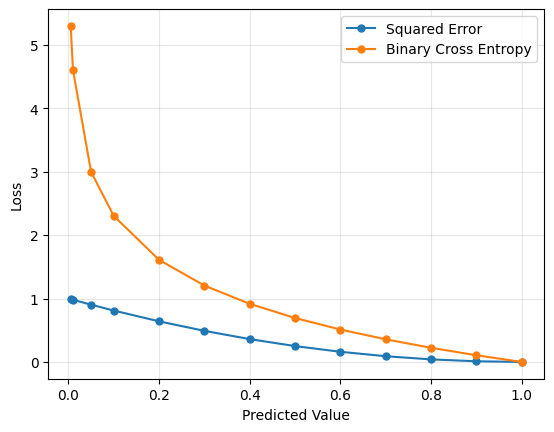
\includegraphics[width=0.9\linewidth]{images/q2_1.png}
		\caption{MSE and BCE loss against predicted value}
		\label{q2_1_img}
	\end{figure}

	\textbf{Question 02} The MSE loss is more appropriate for Application 1 and the BCE loss is more appropriate for Application 2.
	\newline

	For Application 1, where the quantity being predicted is a continuous value, we would like the loss to vary gradually with 
	difference between the predicted value and true value.
	\newline
	
	For Application 2, the goal is to map a continuous value to a binary value based on a certain threshold. In this case, we would like
	to heavily penalize predictions the farther they away below (or above) the threshold, but give little to no penalty for predictions
	on the other side of the threshold, with the hope that it will quickly be forced to the correct side if it happens to land on the
	wrong side.

	\section{Data Pre-Processing}

	\textbf{Question 01} We start by visualizing the distribution of each feature value to decide on a suitable method of scaling. Figure
	\ref{q3_1_1_img} contains plots obtained of the distribution of each feature in the dataset.

	\begin{figure}[H]
		\centering
		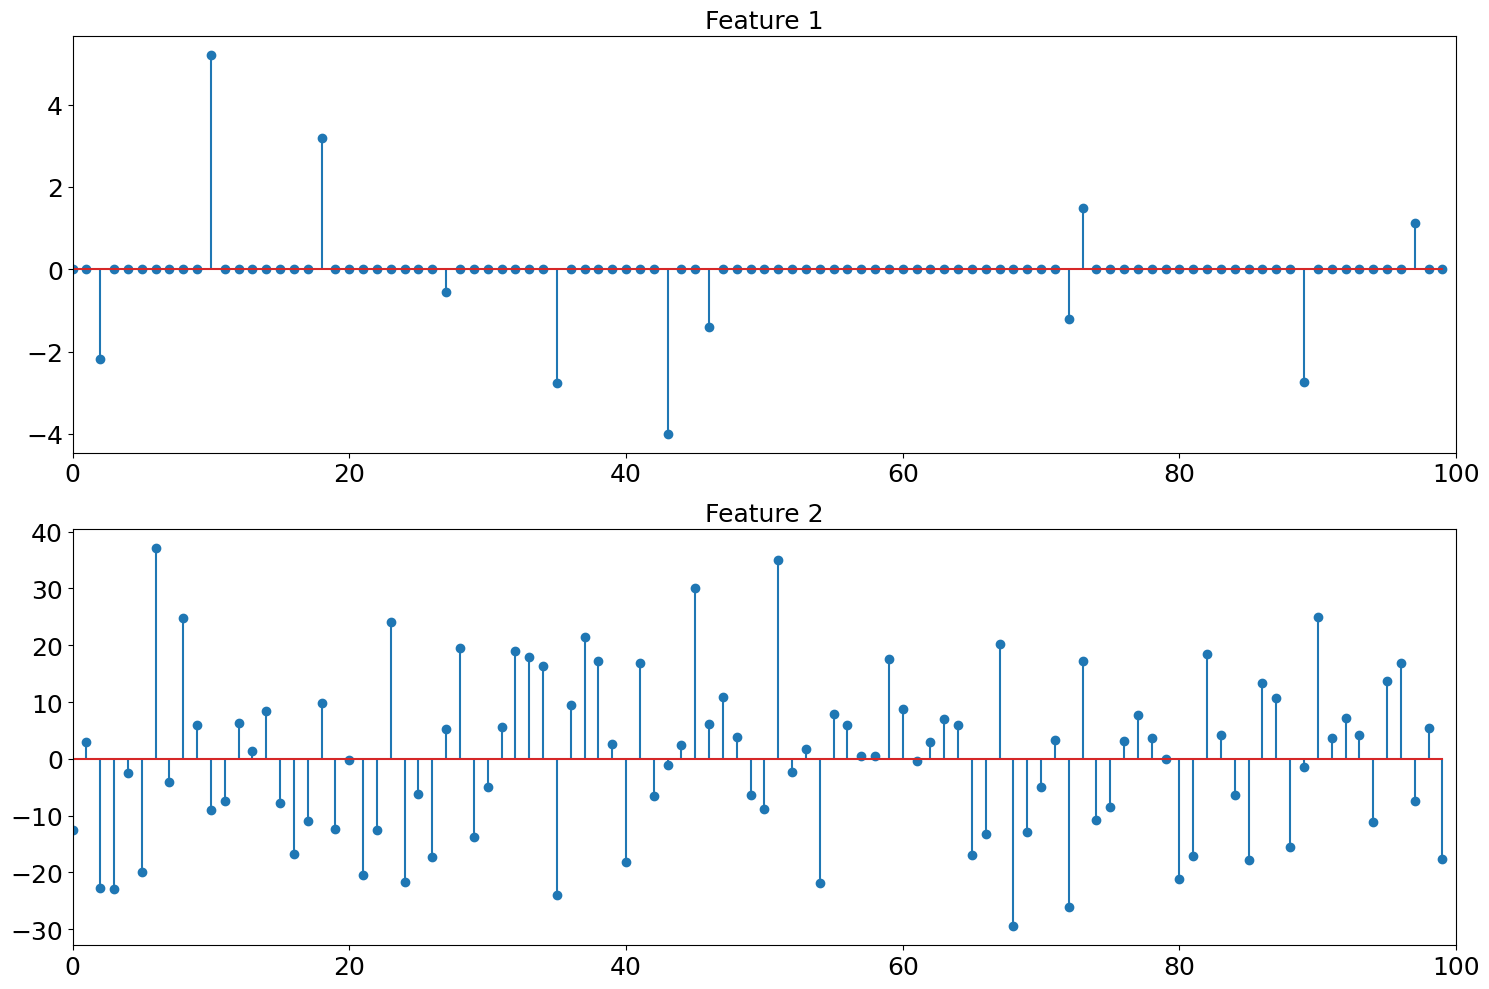
\includegraphics[width=\linewidth]{images/q3_1_1.png}
		\label{q3_1_1_img}
		\caption{Raw values of Feature 1 and Feature 2 for each data point}
	\end{figure}

	We then run the code in Listing \ref{q3_1_code_1} to obtain the following summary statistics of each feature:
	\begin{verbatim}
Feature 1
	 Mean 														: 0.06963158220374253
	 Standard Deviation : 0.751690461643816
	 Maximum 											: 5.2
	 Minimum 											: -2.790493210023752
	 Range 													: 7.990493210023752
Feature 2
	 Mean 														: -0.45935709567298505
	 Standard Deviation : 14.351150951654933
	 Maximum 											: 36.752574877667975
	 Minimum 											: -39.11938330852965
	 Range 													: 75.87195818619762
	\end{verbatim}

	Based on the plots and the summary statistics above, we conclude the following;
	\begin{itemize}[itemsep=1pt]
		\item both features have means close to zero
		\item the features vary on different scales, as they have significantly different standard deviations
		\item both features take on both positive and negative values
		\item Feature 1 is sparsely distributed, with most values being equal to 0
	\end{itemize}

	To bring the values of both features to a similar scale while still preserving the structure and properties of
	each feature, we consider the three following scaling methods;
	\begin{enumerate}[itemsep=1pt]
		\item standard scaling,
		\item min-max scaling, and
		\item max-abs scaling.
	\end{enumerate}
	
	We rule out min-max scaling as it would limit both feature values to a range between 0 and 1, affecting the 
	``symmetric" variation of both feature values among both negative and positive values.
	\newline

	To choose between standard and max-abs scaling, we consider the sparsity of Feature 1.
	\newline
	
	We observe that standard scaling would map zeros of Feature 1 to non-zero values, resulting in a loss of sparsity---a propertsy
	one would likely want to preserve. On the other hand, max-abs scaling would not affect sparsity, as it would map zeros to zeros.
	It also maps to a range between -1 and 1, so negative values map to negative values, and positives to positives.
	\newline

	Hence, we choose max-abs scaling as the method of scaling for both feature values. The code in Listing \ref{q3_1_code_2} implements
	max-abs scaling. Plots of both feature values after such scaling are shown in Figure \ref{q3_1_2_img}.
	
	\begin{figure}[H]
		\centering
		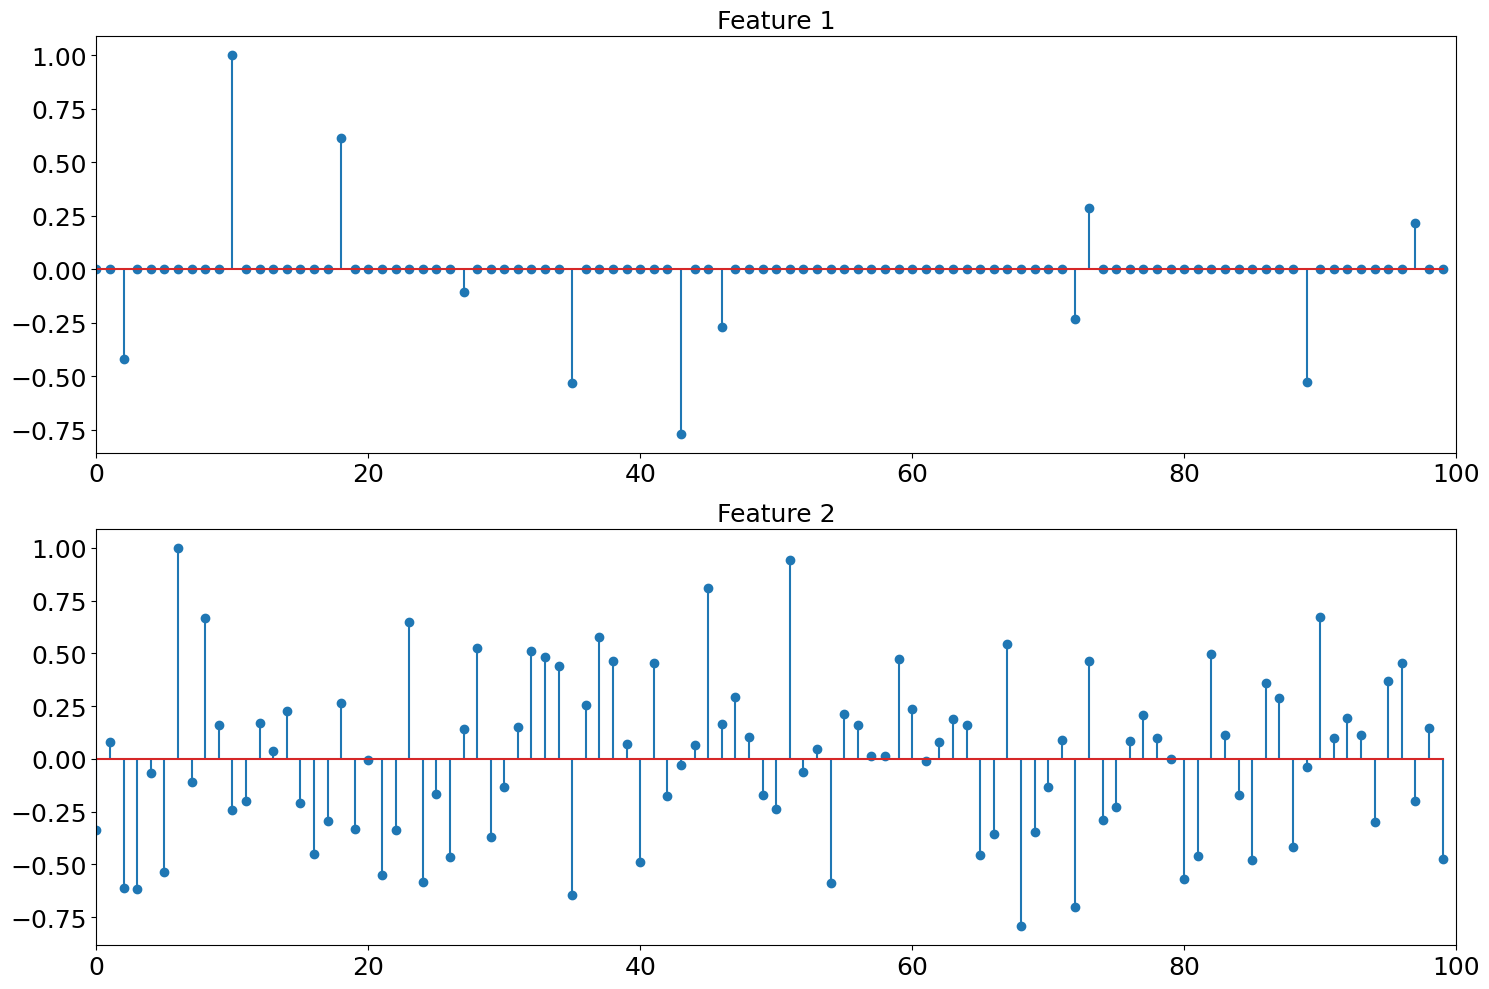
\includegraphics[width=\linewidth]{images/q3_1_2.png}
		\label{q3_1_2_img}
		\caption{Max-abs scaled values of Feature 1 and Feature 2 for each data point}
	\end{figure}
	
	The recalculated summary statistics for the scaled features are as follows:
	\begin{verbatim}
Feature 1 - Max-Abs Scaled
	 Mean 															: -0.007381661238755984
	 Standard Deviation 	: 0.1721201196828633
	 Maximum 												: 1.0
	 Minimum 												: -0.7691686427002166
	 Range 														: 1.7691686427002167
Feature 2 - Max-Abs Scaled
	 Mean 															: 0.00609983651068688
	 Standard Deviation 	: 0.38673155885534527
	 Maximum 												: 1.0
	 Minimum 												: -0.7939711778754481
	 Range 														: 1.7939711778754481
	\end{verbatim}

	\appendix
	\section{Code Snippets}
	\label{code}
		
	\subsection{Impact of Outliers on Linear Regression}

	\subsubsection{Question 02}
	\begin{lstlisting}[label={q1_2_code}, caption={Ordinary Least Squares Regression and Plots}]
# Load the data set
x = np.arange(10).T
y = np.array([20.26, 5.61, 3.14, -30, -40, -8.13, -11.73, -16.08, -19.95, -24.03]).T

# Length of the data set
N = len(x)

# Construct a matrix X with each data point in one row, and each column representing a feature
# The first entry of each row will be 1
X = np.ones((N, 2))
X[:, 1] = x

# We want to choose a matrix of weights w such that (y - xW)^T * (y - xW) is minimized
# The w that minimizes the above--the ordinary least squares weights--is given by
w_OLS = np.linalg.inv(X.T @ X) @ X.T @ y

# Print the learned ordinary least squares weights
print ("Ordinary Least Squares Weights (w):", w_OLS)

# Calculate the prediction for each data point based on the learned w
y_hat = X @ w_OLS

# Plot the original data points and the predicted values
plt.plot(y_hat, label='Predictions', color='red', markevery=x, marker='o', markersize=5)
plt.scatter(x, y, label='Data Points', color='blue')

plt.legend()
plt.xlabel('Independent Variable')
plt.ylabel('Dependent Variable')
plt.grid(True, alpha=0.3)

plt.show()
	\end{lstlisting}

	\subsubsection{Question 04}
	\begin{lstlisting}[label={q1_4_code}, caption={Loss Calculation for Different Models and Values of $\beta$}]
# Set up the weight vectors representing the two given modelss
w_1 = np.array([12, -4])
w_2 = np.array([3.91, -3.55])

# Iterate through each model
for i in range(2):
    w = [w_1, w_2][i]
    print ("Model", i + 1, ":", w)

    # Run the model on the data and find the residuals
    y_hat = X @ w
    residuals = y - y_hat

    # Plot the values predicted by the model
    plt.plot(y_hat, label='Model ' + str(i + 1) + ' Predictions', markevery=x, marker='o', markersize=5)

    # Vary beta through each of the given values and find the loss
    for beta in [1, 1E-6, 1E3]:
        loss = (1 / N) * np.sum((residuals ** 2) / (residuals ** 2 + beta ** 2))
        print ("\t Loss for beta =", "{:<6}".format(beta), ":", loss)
	\end{lstlisting}

	\subsection{Data Pre-Processing}

	\subsubsection{Question 01}
	\begin{lstlisting}[label={q3_1_code_1}, caption={Calculation of Summary Statistics}]
def print_summary_statistics(feature):
    mean = np.mean(feature)
    std_dev = np.std(feature)
    maximum = np.max(feature)
    minimum = np.min(feature)
    range_ = maximum - minimum

    print ("\t Mean \t\t\t:", mean)
    print ("\t Standard Deviation \t:", std_dev)
    print ("\t Maximum \t\t:", maximum)
    print ("\t Minimum \t\t:", minimum)
    print ("\t Range \t\t\t:", range_)

for i in range(2):
    feature = [sparse_signal, epsilon][i]

    print ("Feature", i + 1)
    print_summary_statistics(feature)
	\end{lstlisting}

	\begin{lstlisting}[label=q3_1_code_2, caption={Max-Abs Scaling}]
def max_abs_scale(feature):
    max_abs = np.max(np.abs(feature))
    if max_abs == 0: # Avoid division by zero
        return feature
    return feature / max_abs
	\end{lstlisting}

\end{document}